% For instructions,
\documentclass[reprint, amsmath, amssymb, aps]{revtex4-2}

%\usepackage[norsk]{babel}
%Uncomment this if you want to write in Norwegian

\usepackage{graphicx}% Include figure files
\usepackage{dcolumn}% Align table columns on decimal point
\usepackage{bm}% bold math
\usepackage{hyperref}% add hypertext capabilities
\usepackage{booktabs}
\usepackage{float}
\usepackage{siunitx}



\begin{document}
\title{Project2 - FYS4460}
\author{Mikkel Metzsch Jensen}

\date{\today}
\maketitle

\subsection*{f) Estimate n}
Remove "percolating cluster"?.



\begin{figure}[H]
  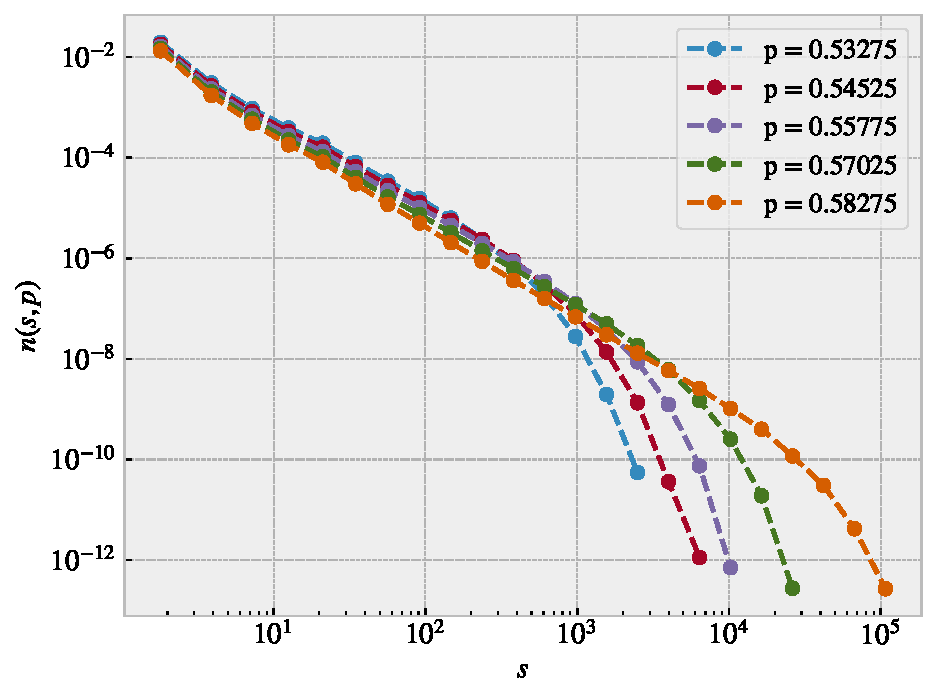
\includegraphics[width=\linewidth]{figures/f_p_below.pdf}
  \caption{$n(s,p)$ with $p$ approaching $p_c = 0.59275$ from below in a $L \times L = 1000 \times 1000$ system. The results are averaged over 300 Monte Carlo cycles with a logaritmic binsize of $1.6^i$ for bin $i$.}
  \label{fig:f}
\end{figure}

\begin{figure}[H]
  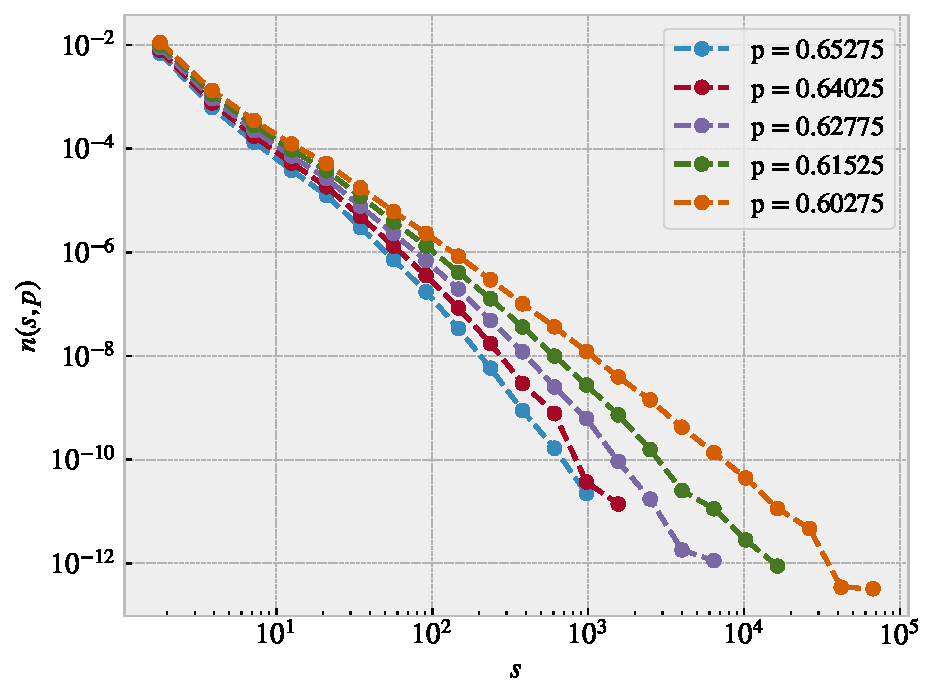
\includegraphics[width=\linewidth]{figures/f_p_above.pdf}
  \caption{$n(s,p)$ with $p$ approaching $p_c = 0.59275$ from above in a $L \times L = 1000 \times 1000$ system. The results are averaged over 300 Monte Carlo cycles with a logaritmic binsize of $1.6^i$ for bin $i$.}
  \label{fig:f}
\end{figure}

\subsection*{g)}

Antagelse
\begin{align*}
  n(s,p) = s^{-\tau}F\left(\frac{s}{s_\xi}\right), \quad s_\xi \propto |p - p_c|^{-1/\sigma}
\end{align*}

\begin{figure}[H]
  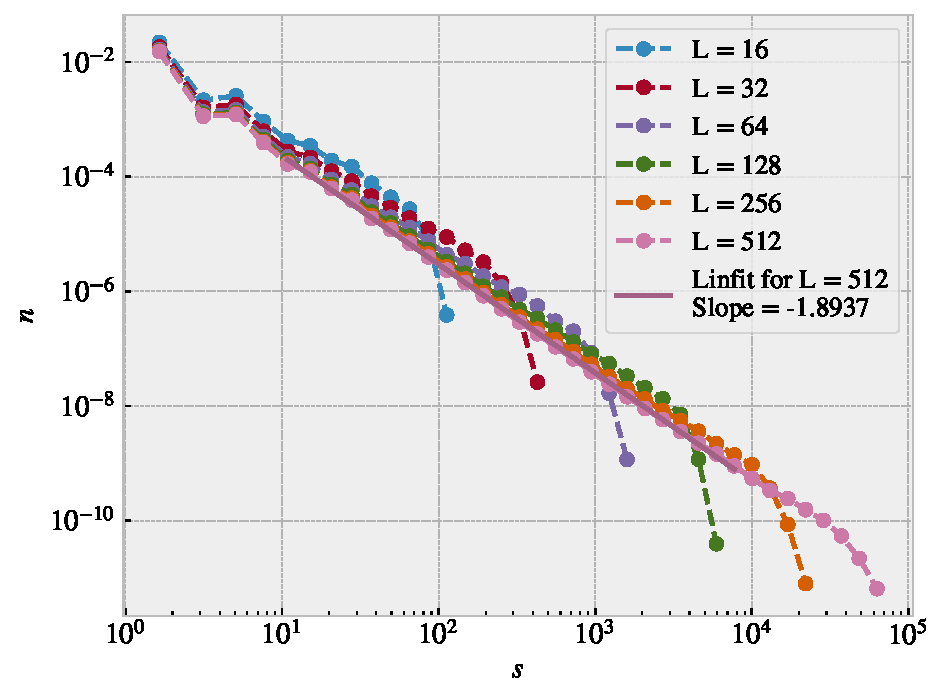
\includegraphics[width=\linewidth]{figures/g.pdf}
  \caption{$n(s,p)$ with $p = p_c = 0.59275$ with $L = 2^k$ for $k = 4, \cdots, 9$ The results are averaged over 1000 Monte Carlo cycles with a logaritmic binsize of $1.1^i$ for bin $i$. By making a linear fit on the first part of the datapoints for $L = 512$ we estimate $\tau$ as $1.89$.}
  \label{fig:g}
\end{figure}

Result from book is $\tau_{book} = 187/91 \approx 2.05$ giving a relative error
\begin{align*}
  \eta_\tau= \left|\frac{187/91 - 1.89}{1.89}\right| = 0.087
\end{align*}


\subsection*{h)}


\begin{figure}[H]
  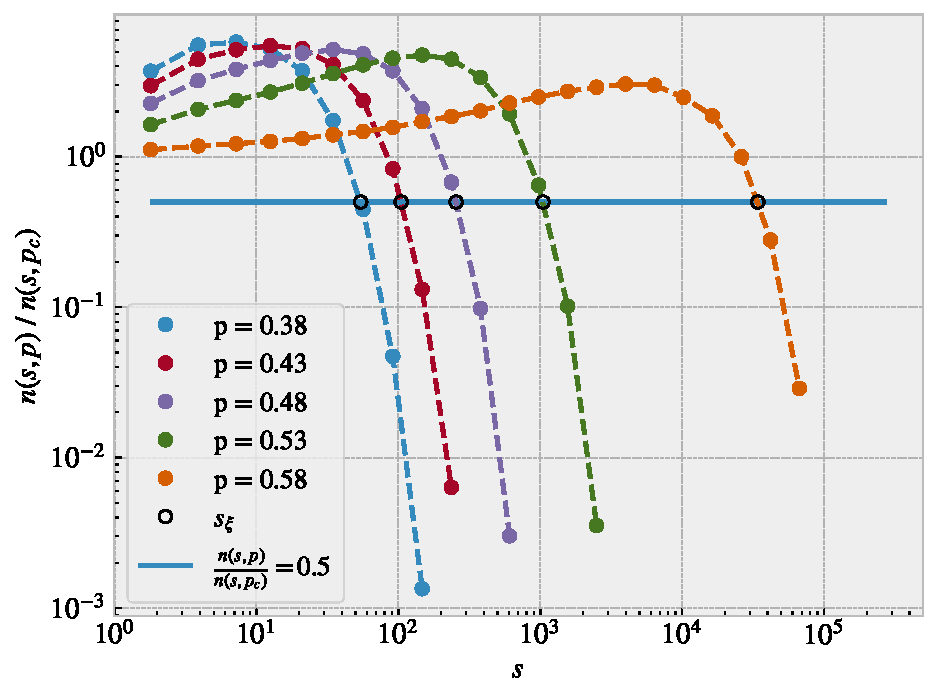
\includegraphics[width=\linewidth]{figures/h_n_over_nc.pdf}
  \caption{L = 1000, MC = 500, a = 1.6}
  \label{fig:h_n_over_nc.pdf}
\end{figure}

\begin{figure}[H]
  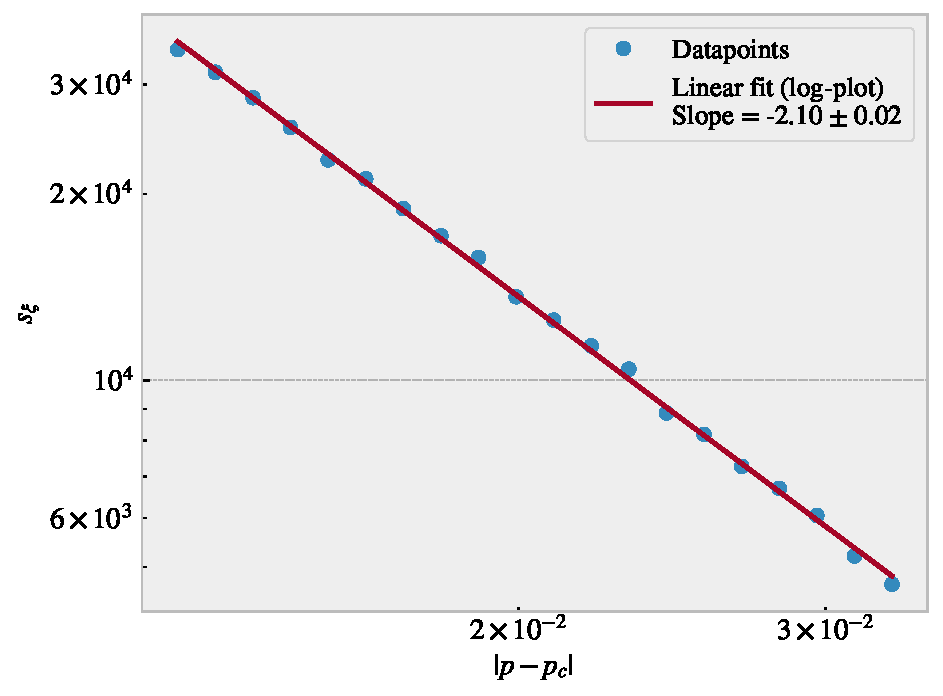
\includegraphics[width=\linewidth]{figures/h_sigma.pdf}
  \caption{$s_{\xi}$ defined as $n(s,p)/n(s,p_c) = F(s/s_{\xi}) = 0.5$ as a function of $|p-p_c|$ for 20 equally distributed values in the interval $p \in [0.56, 0.58]$. For each value of $p$ we used a system size of $L = 1000$, a logaritmic binsize of $1.6^i$ for bin $i$ and averagede the result for 500 MC cycles. Notice that choosing $0.58 < p \le p_c$ gave more unreliable results as the relations diverges near $p_c$}
  \label{fig:h}
\end{figure}
From the linear fit on \ref{fig:h} we find
\begin{align*}
  \sigma = -\frac{1}{\text{slope}} =  0.475 \pm 0.004
\end{align*}
By experience I found the second decimal to vary beetween runs and reduce my estimate to
\begin{align*}
  \sigma = 0.4(8)
\end{align*}
Result from book is $\sigma_{book} = 36/91 \approx 0.40$ giving a relative error
\begin{align*}
  \eta_\sigma = \left|\frac{36/91 - 0.48}{0.48}\right| = 0.18
\end{align*}

\subsection*{i)}
Handles multiple spanning cluster by mean value.

\begin{figure}[H]
  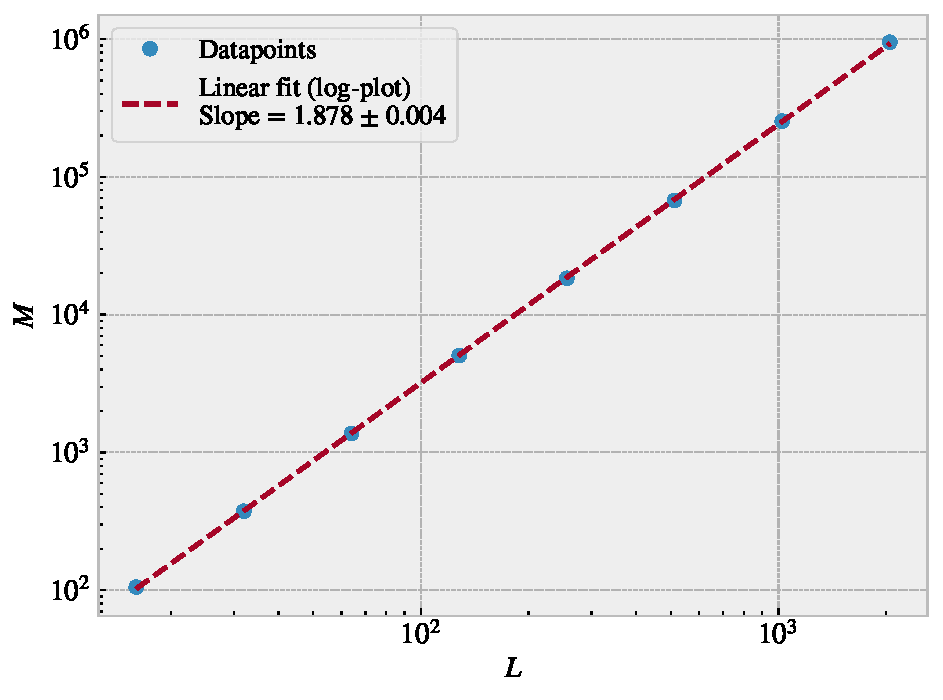
\includegraphics[width=\linewidth]{figures/i.pdf}
  \caption{$MC_cycles = 500$}
  \label{fig:i}
\end{figure}
We find that $M(L)$ goes as
\begin{align*}
  M = L^D, \qquad D = 1.878 \pm 0.03
\end{align*}
Result from book is $D_{book} = 91/48 \approx 1.896$ giving a relative error
\begin{align*}
  \eta_D= \left|\frac{91/48 - 1.878}{1.878}\right| = 0.009
\end{align*}




\begin{thebibliography}{9}
  \bibitem{compendium}
\end{thebibliography}

\end{document}
